\documentclass[11pt]{book}
\usepackage[colorlinks = true,linkcolor = blue]{hyperref}
\usepackage[letterpaper]{geometry} % Custom margins
\usepackage{graphicx}
\usepackage[spanish]{babel}
\usepackage[T1]{fontenc}
\usepackage[utf8]{inputenc}
\usepackage{remreset}

\makeatletter
  \@removefromreset{section}{chapter}
\makeatother
%\usepackage[dvipsnames]{xcolor} % Required for custom color
\usepackage{color,colortbl}
\usepackage[utf8]{inputenc}
\usepackage{geometry} % Custom margins
\usepackage[spanish]{babel}
\usepackage{adjustbox,dashbox}
\usepackage{array}
\usepackage{tikz,pgfplots,pgfkeys}
\usepackage{forest,mathtools,siunitx}
\usepackage{amsfonts, amssymb, amsxtra, amsmath, amsbsy}
\usepackage{newclude}
\usepackage{ifthen}
\usepackage{float}
\usepackage{fancybox}
\usepackage{graphicx,tabularx}
\usepackage{multicol,multirow}
\usepackage{enumitem} % Customising the numbered lists
\usepackage{xhfill} % Making the pink block not extend beyond the margin
\usepackage{nameref} % reference the names of the sections
\usepackage{caption,capt-of}
\usepackage[normalem]{ulem} % Dashed lines in appendix
\usepackage{ragged2e} % Ragged left
\usepackage{booktabs}
\usepackage[unboxed]{cwpuzzle}
\usepackage[colorlinks = true,linkcolor = blue]{hyperref}
\usepackage{subfiles}
\usepackage{wrapfig}
\input{insbox}
\usepackage{etoolbox}
\usepackage{mwe}
\usepackage{comfortaa}
\usepackage[T1]{fontenc}
\renewcommand*\oldstylenums[1]{{\firaoldstyle #1}}
\usepackage[T1]{fontenc}
\usepackage{pythontex}
\usepackage{polynom}
\usepackage{longdivision}

 
\renewcommand{\thechapter}{Unidad \arabic{chapter}}
\renewcommand{\thesection}{S\arabic{section}}
\renewcommand{\thesubsection}{L\arabic{subsection}}
\setlength{\parindent}{0pt}

\begin{document}
\pagestyle{empty}
\newgeometry{letterpaper,left=15mm,top=50mm,bottom=0mm} % Custom margins
\begin{center}
  {\Huge F\'isica}\\
  \vspace{2cm}
  \normalsize
  \textbf{\large Cuaderno de trabajo}\\
  para los alumnos de 2$^\circ$ de  Secundaria\\
  en el curso durante el ciclo escolar\\
  \textbf{2022-2023}\\
  \vspace{2.5cm}
  \small POR\\
  \Large J. C. Melchor Pinto\\[0.5em]
  \normalsize Profesor de asignatura en\\
  \vspace{1cm}
  
\includegraphics[width=4cm]{./Unidad 2/Images/LOGO_RDS_nobg}
\end{center}
\vspace{2cm}
%\include*{Functional/TitlePage}
\hspace{-16mm}
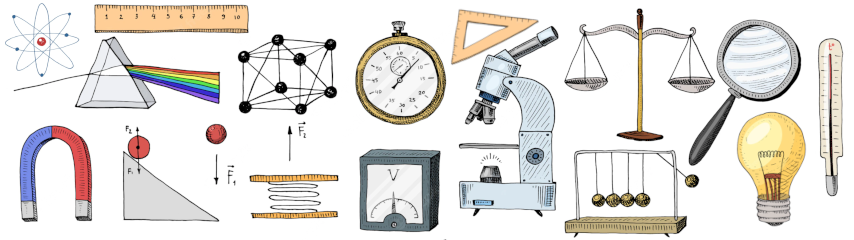
\includegraphics[width=\paperwidth]{./Unidad 2/Images/cover_bg}
\restoregeometry
\tableofcontents
\chapter{}



\end{document}






